\section{Semaine 22 : 03/07/2023 - 07/07/2023}
\graphicspath{{semaines/semaine_22/images/}}

\begin{abstract}
	Après discussion avec Emmanuel, il aimerait que je refasse les mêmes tests sur un carré.
	
	Cette semaine, j'ai également bien avancer sur le rapport. J'ai également implémenter la conversion du rapport latex en fichiers antora et ait commencé la CI sur github.
\end{abstract}

\subsection{Résultats sur le carré}

On considère ici la solution analytique suivante
$$u_{ex}(x,y)=S\times\sin(2\pi fx+p)\times\sin(2\pi fy+p)$$
avec $S=0.5$, $f=1$ et $p=0$. Solution \textbf{homogène} sur notre domaine, le carré $[0,1]^2$. On prendra $\mathcal{O}=[-0.5,1.5]^2.$

\subsubsection*{Dérivées}

Voici les dérivées premières obtenus avec tensorflow :

\begin{minipage}{\linewidth}
	\centering
	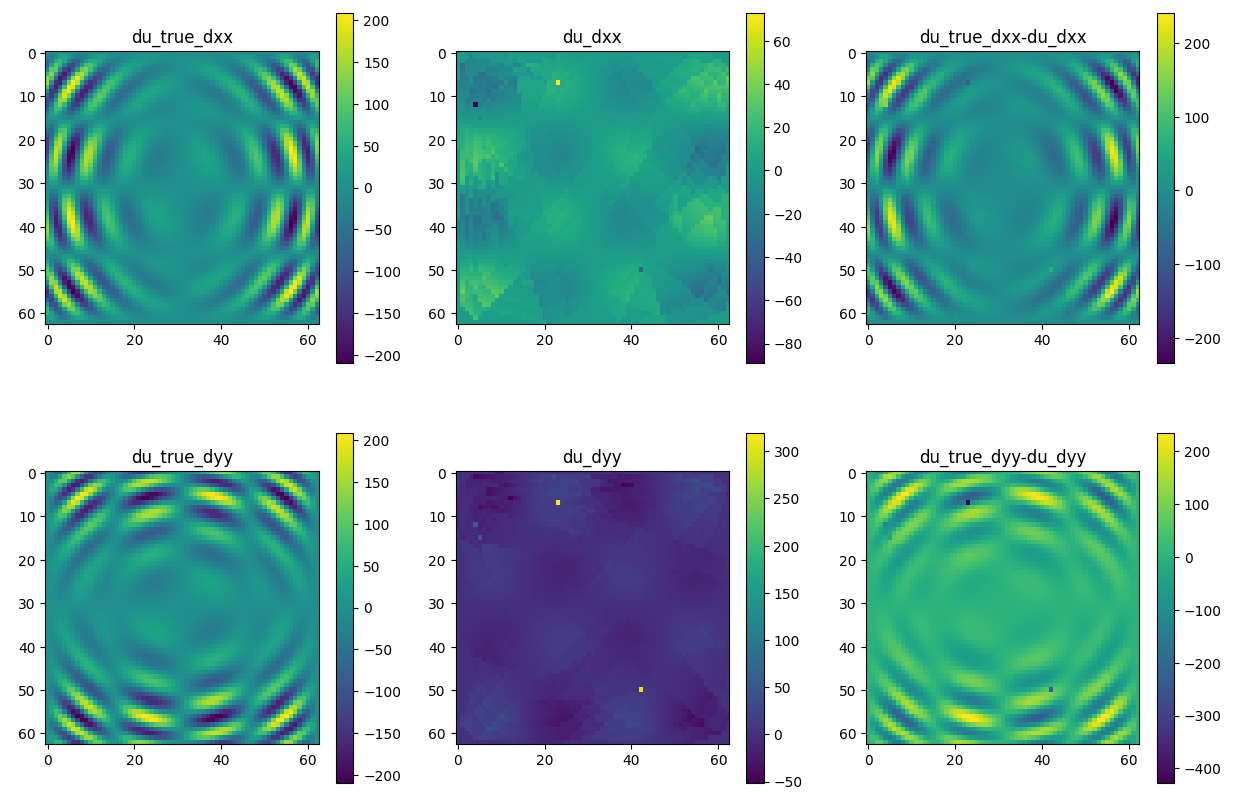
\includegraphics[width=0.65\linewidth]{Dérivées_exactes_1.png}
\end{minipage}

Voici les dérivées premières obtenus avec FEniCS :

\begin{minipage}{\linewidth}
	\centering
	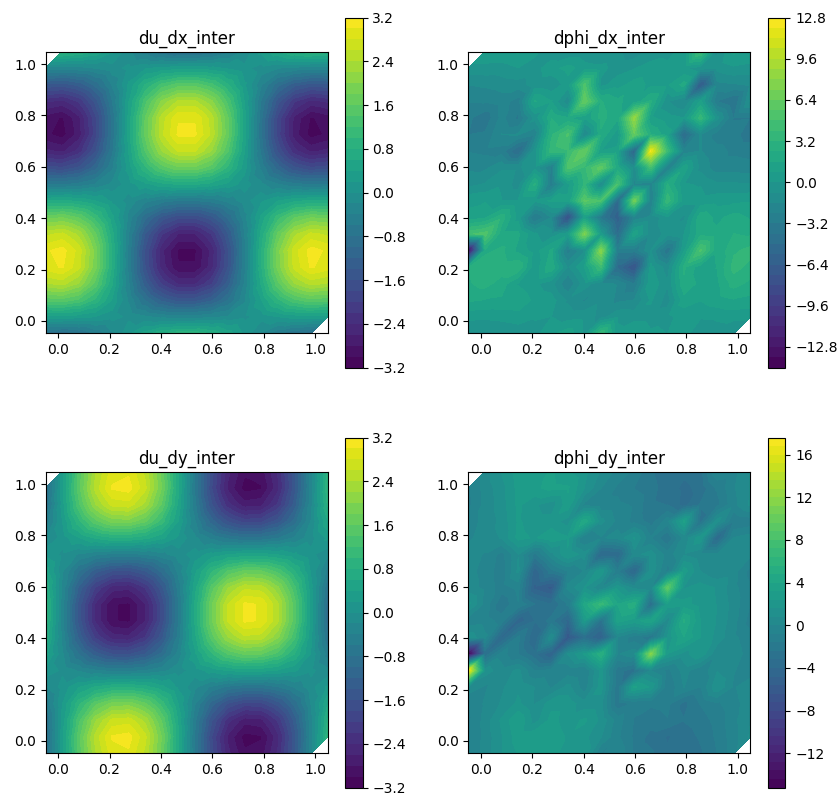
\includegraphics[width=0.5\linewidth]{Dérivées_FEniCS_1.png}
\end{minipage}

\subsubsection*{Comparaison FEM-PhiFEM}

\begin{minipage}{\linewidth}
	\centering
	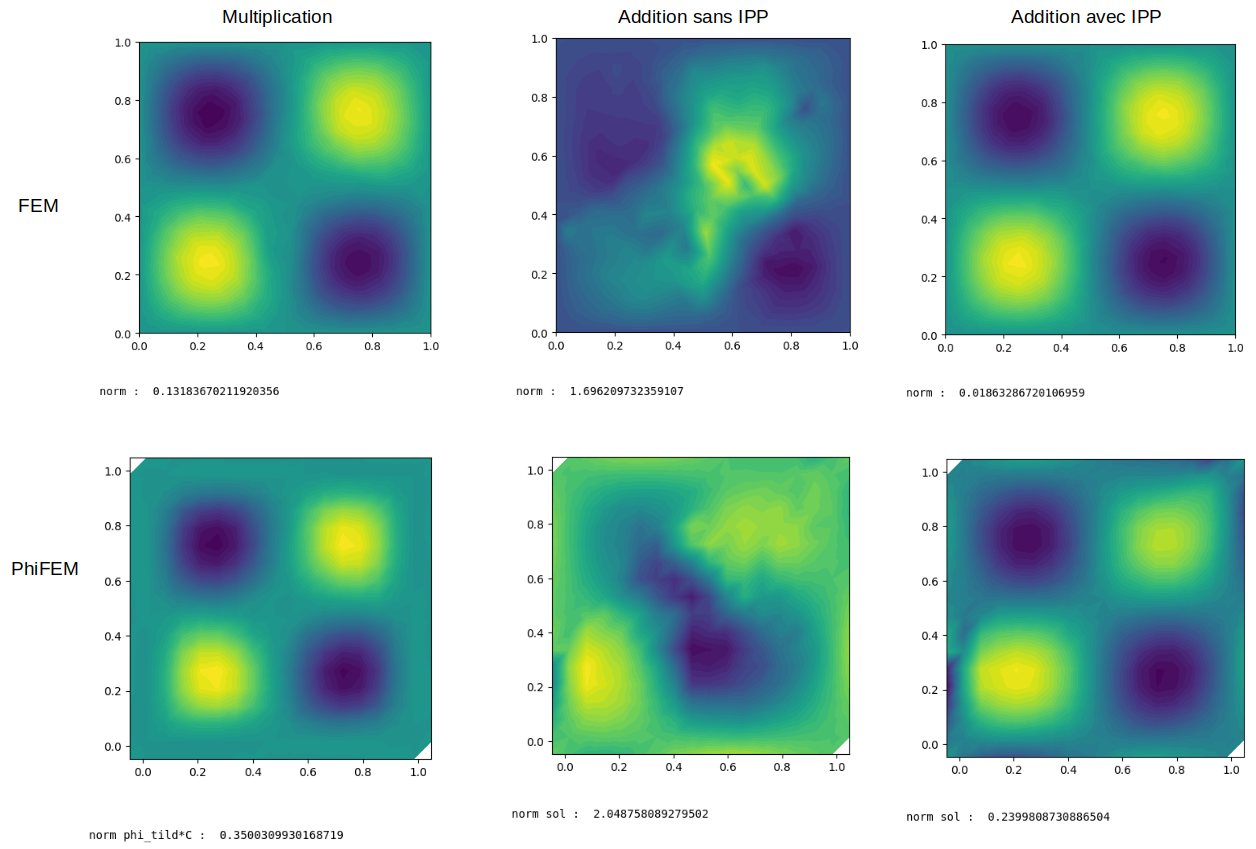
\includegraphics[width=0.9\linewidth]{FEM_vs_PhiFEM.png}
\end{minipage}